\section{Infrared Thermography}

Infrared tomography is a imaging technique that utilizes infrared radiation emitted from different objects. 
The existence of infrared radiation was first discovered in 1800 by Sir Frederick William Herschel. 
His experiments lead to the knowledge that any object above absolute zero emits energy-electromagnetic radiation depending on its temperature. The human body has a temperature around 37 degrees, and the emitted radiation energy is in the infrared region.\cite{ignacio2017} 

\subsection{Physical principals}

Infrared thermography is commonly used to calculate surface temperatures and to do this it is important to understand and define the concepts of heat and temperature.\cite{ignacio2017} 

Heat is the energy that passes from a warm object to another object that is cooler than its own. A warm object will decrease in internal energy and a cold will increase due to the temperature difference and therefore the heat transfer. 
Temperature is a measure for the internal energy within an object and can be defined at the average kinetic energy of the object.\cite{ignacio2017} 

\textbf{Electromagnetic radiation}
Electromagnetic radiation is a propagation of energy trough a medium without the transportation of a mass. An electromagnetic wave is made of the relationship between frequency (f), wavelength ($\lambda$) and the speed of light (c). This is stated in the equation of wave motion.\cite{ignacio2017}  
\begin{flalign}
	\lambda = \frac{c}{f}
	\label{eq:wave}
\end{flalign}
Depending on the frequency and wavelength certain characteristics arise an form what i called the electromagnetic spectrum. The electromagnetic spectrum is the electromagnetic energy that is emitted. This extends from radiation of low energy such as radio waves and infrared, to waves of higher energy in form of eg. X-rays. A graphical representation of the electromagnetic spectrum can be seen on \cref{fig:em_spectrum}.\cite{ignacio2017}        

\begin{figure}[H]                                         
	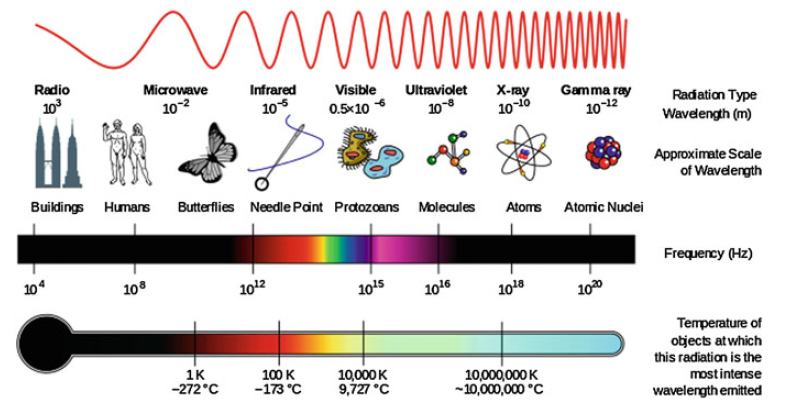
\includegraphics[width=.66\textwidth]{figures/em_spectrum}  
	\caption{The electromagnetic spectrum with wavelength, emitters, frequency and temperature.\cite{ignacio2017}  }
	\label{fig:em_spectrum}  
\end{figure}   
 
Infrared radiation is also known as thermal radiation because the relationship between temperature and infrared radiation. Infrared radiation have a wavelength from 769nm to 1mm. Thermal radiation is emitted when the temperature of the object is close to the environmental temperature.\cite{ignacio2017}  

The black body cencept

\subsection{Measuring thermal energy}

Measuring thermal radiation uses the knowledge that electromagnetic radiation is proportional to the internal energy. With a lens, the radiation beam emitted, is focused on to a detector element that generates an electric output proportional to the radiation.\cite{optris2009}

\begin{figure}[H]                                         
	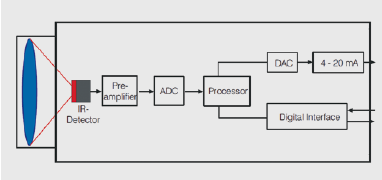
\includegraphics[width=.55\textwidth]{figures/IR_cam}  
	\caption{Simplified block diagram of an standard infrared camera.\cite{optris2009}}
	\label{fig:em_spectrum}  
\end{figure} 

extra notes that i'we just copied that we can use later 

The advantages of non-contact temperature measurement
are obvious – it supports:
• Temperature measurements of moving or overheated
objects and of objects in hazardous surroundings
• Very fast response and exposure times
• Non-interactive measurement, no influence on
the measuring object
• Non-destructive measurement
• Measurement point durability, no mechanical wear


